\documentclass[]{scrartcl}

\usepackage{amsmath}
\usepackage{amssymb}
\usepackage[utf8]{inputenc}
\usepackage[T1]{fontenc}
\usepackage{lmodern}
\usepackage{ngerman}
\usepackage{geometry}
\usepackage{graphicx}
\usepackage{wrapfig}
\usepackage{caption}
\usepackage{wasysym}
\usepackage{siunitx}
\usepackage{picinpar}
\usepackage{tikz}
\usepackage{float}

\renewcommand{\figurename}{Abb.}
\usepackage[
	colorlinks=true,
	urlcolor=blue,
	linkcolor=black
]{hyperref}


%Hier Titel und so
\newcommand{\versuchnummer}{V59} 
\newcommand{\versuchname}{Modulation und Demodulation elektrischer Schwingungen} 
\newcommand{\versuchdatum}{24.02.16} 


\title{Versuch \versuchnummer\\ \versuchname}
\subtitle{Physikalisches Fortgeschrittenenpraktikum}
\author{Robert Rauter und Björn Lindhauer}
\date{\versuchdatum} 
\begin{document}
\begin{titlepage}
{\large \versuchdatum}
\vspace{7cm}
\begin{center}
\textbf{\huge Versuch \versuchnummer:}\\
\vspace{0.5cm}
\textbf{\huge \versuchname}\\
\vspace{0.2cm}
\textbf{ Physikalisches Fortgeschrittenenpraktikum}\\
\vspace{9cm}

{\Large Robert Rauter \ \ \hspace{1.5cm} und \hspace{1.5cm} Björn Lindhauer}\\
{ \url{robert.rauter@tu-dortmund.de} \ \ \hspace{2cm} \url{bjoern.lindhauer@tu-dortmund.de}}
\end{center}
\end{titlepage}
\section{Einleitung}
Unter Modulation wird Veränderung der Amplitude, der Phase oder der Frequenz einer Welle im Rhythmus des Nachrichtensignals verstanden. Sie wird benötigt, um Signale mit elektromagnetische Wellen zu übertragen.\\
Das übertragene Signal muss beim Empfänger anschließend zurück gewonnen werden. Dieser Vorgang wird als Demodulation bezeichnet.\\ Mit der Zeit wurden verschiedene Verfahren mit unterschiedlichen Stärken und Schwächen in der Störsicherheit, im Wirkungsgrad, in der Verzerrungsfreiheit und in der Breite des Frequenzspektrums entwickelt. Diese Verfahren lassen sich in zwei Klassen, den Amplitudenmodulations- und Phasenwinkelmodulation- Verfahren unterteilen.\\
In diesen Versuch sollen Beispiele beider Verfahrensklassen untersucht werden.
\section{Theoretische Grundlagen}
\subsection{Amplitudenmodulation}
Eine Amplitudenmodulation kann durch eine hochfrequente Trägerschwingung $U_{\text{T}}\left(t\right)$ mit niederfrequenten Modulationssignal $U_{\text{M}}\left(t\right)$ erreicht werden.\\
Die zeitliche Entwicklung der Amplituden lassen sich durch
\begin{align}
U_{\text{T}}\left(t\right)=\hat{U}_{\text{T}} \cos \omega_{\text{T}}t  \text{ und }U_{\text{M}}\left(t\right)=\hat{U}_{\text{M}} \cos \omega_{\text{M}}t
\end{align}
darstellen. Dabei sind die $\omega_{i}$ jeweils die Frequenzen und $\hat{U}_{i}$ die Amplituden der Trägerschwingung bzw. der Modulationsschwingung.\\
Daraus folgt für die amplitudenmodulierte Schwingung
\begin{align}
U_3\left(t\right)=\hat{U}_{\text{T}} \left(1+m\cos \omega_{\text{M}}t\right)\cos \omega_{\text{T}}t
\label{eq:amplitudederamplitudenmoduliertenschwingung}
\end{align}
mit den Modulationsgrad genannten Größe
\begin{align}
m=\gamma \hat{U}_{\text{M}} \hspace{0.5cm}\text{.}
\end{align}
Der Modulationsgrad kann nur Werte zwischen 0 und 1 annehmen, sodass die Maxima der modulierten Schwingung zwischen $\hat{U}_{\text{T}}\left(1-m\right)$ und $\hat{U}_{\text{T}}\left(1+m\right)$ liegen, wie in Abbildung 
\ref{fig:zeitabhaengigkeit_momentanspannung} anschaulich dargestellt.
Die Gleichung \ref{eq:amplitudederamplitudenmoduliertenschwingung} lässt sich durch trigonometrischer Beziehungen in die Form
\begin{align}
U_3\left(t\right)=\hat{U}_{\text{T}}\left(\cos \omega_{\text{T}}t+ \frac{m}{2}\cos \left( \omega_{\text{T}}+\omega_{\text{M}}\right)t +\frac{m}{2}\cos \left( \omega_{\text{T}}-\omega_{\text{M}}\right)t  \right) 
\label{eq:amplitudederamplitudenmoduliertenschwingungbesser}
\end{align}
überführen, anhand jener das Frequenzspektrum einfach abgelesen werden kann. Das Spektrum besteht aus 3 Linien bei den Frequenzen $\omega_{\text{T}}$, $\omega_{\text{T}}+\omega_{\text{M}}$ und $\omega_{\text{T}}-\omega_{\text{M}}$ und ist Beispielhaft in Abbildung \ref{fig:frequenzsprektum_amplitudenmodulierten} dargestellt.\\
Besteht die Modulationsspannung $\hat{U}_\text{M}$ aus einer Reihe von verschiedener Frequenzen, so verbreitern sich die beiden äußeren Linien zu Frequenzbändern.\\
\begin{figure}[H]
\centering 
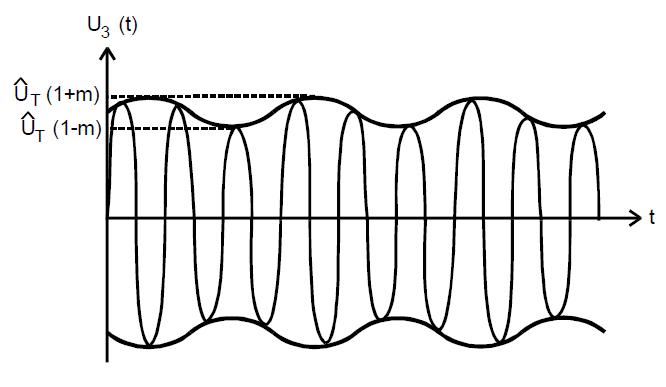
\includegraphics[width=10cm]{images/zeitabhaengigkeit_momentanspannung.png}
\caption{Zeitliche Darstellung der Momentanspannung $U_3$ nach Gleichung \ref{eq:amplitudederamplitudenmoduliertenschwingung} (1)}
\label{fig:zeitabhaengigkeit_momentanspannung}
\end{figure}
In Gleichung \ref{eq:amplitudederamplitudenmoduliertenschwingungbesser} ist ersichtlich, dass das Signal bei $\omega_\text{T}$ keinerlei Informationen besitzt, da sie unabhängig von $\hat{U}_\text{M}$ ist. Es wird auch als Trägerabstrahlung bezeichnet und stellt in der Praxis nur einen unnötigen Energieverbrauch da und wird deswegen vermieden.\\
Es kann außerdem Energie gespart werden, indem eines der beiden Bänder durch ein Bandfilter unterdrückt wird. Dies wird auch Einseitenbandmodulation genannt. Es ist möglich, da die beiden Bänder die selbe Information enthalten.
\begin{figure}[H]
\centering 
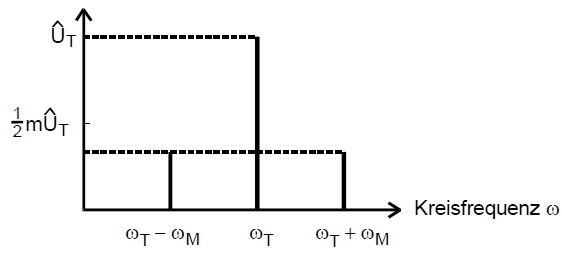
\includegraphics[width=10cm]{images/frequenzsprektum_amplitudenmodulierten.png}
\caption{Frequenzspektrum einer nach \ref{eq:amplitudederamplitudenmoduliertenschwingungbesser} amplitudenmodulierten Schwingung (1)}
\label{fig:frequenzsprektum_amplitudenmodulierten}
\end{figure}
Die Amplitudenmodulation besitzt jedoch eine geringe Störsicherheit und Verzerrungsfreiheit.
\subsection{Frequenzmodulation}\label{sec:frequenzmodulation}
Bei der Frequenzmodulation wird nicht die Amplitude, sondern die Frequenz im Rhythmus des Modulationssignales geändert.\\
Es ergibt sich ein Signal der Form
\begin{align}
U\left(t\right)=\hat{U}\sin \left( \omega_{\text{T}}t+ m \frac{\omega_{\text{T}}}{\omega_{\text{M}}}\cos \omega_{\text{M}}t \right)\label{eq:frequenzmodulationsignal}
\end{align}
mit den Modulationsgrad $m$, der durch die Modulationsspannung gegeben ist.\\
Durch Ableitung des Arguments der Sinus-Funktion in \ref{eq:frequenzmodulationsignal} kann die Momentanfrequenz
\begin{align}
f\left(t\right)=\frac{\omega_{\text{T}}}{2\pi}\left(1+m\sin \omega_{\text{M}}t\right)
\end{align} 
bestimmt werden.\\
Des weiteren wird die Größe $m\frac{\omega_{\text{T}}}{2\pi}$ als Frequenzhub bezeichnet und gibt die Variationsbreite der Schwingungsfrequenz an.\\
Wie ein frequenzmoduliertes Signal aussehen könnte, ist in Abbildung
\ref{fig:frequenzmodulation_beispiel} abgebildet.
\begin{figure}[H]
\centering 
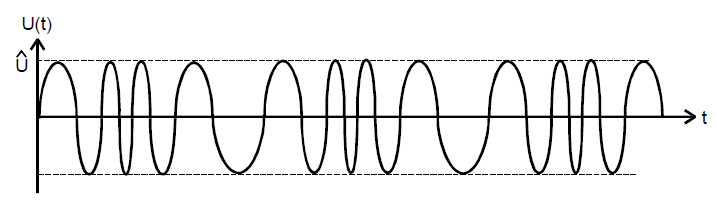
\includegraphics[width=13cm]{images/frequenzmodulation_bsp.png}
\caption{Beispielhafter zeitlicher Verlauf eines frequenzmodulierten Signals (1)}
\label{fig:frequenzmodulation_beispiel}
\end{figure} 
Es soll im folgenden nur die Schmalband-Frequenzmodulation betrachtet werden, mit niedrigen Frequenzhub, sodass
\begin{align}
m\frac{\omega_{\text{T}}}{\omega_{\text{M}}}\ll 1 \label{eq:frequenzmodulationsignalentwicklungsparameter}
\end{align}
ist und \ref{eq:frequenzmodulationsignal} nach dieser Größe entwickelt werden kann. Dazu wird \ref{eq:frequenzmodulationsignal} zunächst durch Additionstheoreme in die Form
\begin{align}
U\left(t\right)=\hat{U}\left(\sin   \omega_{\text{T}}t \cos\left(m \frac{\omega_{\text{T}}}{\omega_{\text{M}}}\cos \omega_{\text{M}}t \right)+\cos   \omega_{\text{T}}t \sin\left(m \frac{\omega_{\text{T}}}{\omega_{\text{M}}}\cos \omega_{\text{M}}t \right) \right)\label{eq:frequenzmodulationsignalentwicklungsform}
\end{align}
gebracht, da diese sich leichter nach \ref{eq:frequenzmodulationsignalentwicklungsparameter} entwickeln lässt.\\
Die entstehende Gleichung
\begin{align}
U\left(t\right)=\hat{U}\left(\sin   \omega_{\text{T}}t+ \frac{m}{2}\frac{\omega_{\text{T}}}{\omega_{\text{M}}}\cos\left(\omega_{\text{T}}+\omega_{\text{M}}\right) +\frac{m}{2}\frac{\omega_{\text{T}}}{\omega_{\text{M}}}\cos\left(\omega_{\text{T}}-\omega_{\text{M}}\right)  \right)
\end{align}
hat die gleiche Form wie die Gleichung \ref{eq:amplitudederamplitudenmoduliertenschwingungbesser} beim amplitudenmodulierte Signal und besteht auch aus drei Teilschwingungen, jedoch sind die Seitenlinien um $90^\circ$ gegen die Trägerschwingung in der Phase verschoben.\\
Bei starker Frequenzmodulation mit
\begin{align}
m \omega_{\text{T}} \approx \omega_{\text{M}}
\end{align}
muss die Entwicklung von \ref{eq:frequenzmodulationsignalentwicklungsform} um höhere Ordnungen ergänzt werden.\\
Dabei ergibt sich die Darstellung
\begin{align}
U\left(t\right)=\hat{U}\sum\limits_{n=-\infty}^{\infty} J_n\left(m\frac{\omega_{\text{T}}}{\omega_{\text{M}}} \right)\sin \left(\omega_{\text{T}}+n\omega_{\text{M}}\right)t\label{eq:frequenzmodulation_bessel}
\end{align}
mit der Besselsche Funktion $J_n\left(x\right)$. Dabei wird das Frequenzspektrum in Falle eines hohen Modulationsgrades vollständig abgedeckt, wie es aus Gleichung \ref{eq:frequenzmodulation_bessel} hervorgeht. In praktischen Anwendungen müssen jedoch nur Frequenzen nahe $\omega_{\text{T}}$ betrachtet werden, da die Besselsche Funktion für $x\l 1$ schnell abfällt.   
\subsection{Modulationsschaltungen}
\subsubsection*{Amplitudenmodulation}
Um eine Amplitudenmodulation zu erreichen, muss das Produkt zweier Spannungen gebildet werden. Dafür wird ein Bauteil mit nicht-linearer Kennlinie benötigt.\\
Die einfachste Modulationsschaltung besteht aus einer Diode und den zwei Spannungsquellen und ist in Abbildung \ref{fig:einfachemodulation} skizziert.
\begin{figure}[H]
\centering 
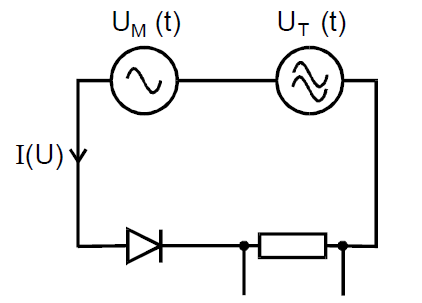
\includegraphics[width=8cm]{images/primitive_modulationsschaltung.png}
\caption{Einfache Modulationsschaltung mit einer Diode (1)}
\label{fig:einfachemodulation}
\end{figure} 
Die Amplitudenmodulation dieser Schaltung wird ersichtlich, wenn der Strom
\begin{align}
I\left(U\right)=a_0+a_1 U+a_2U^2 + O(U^3)
\end{align}
nach $U$ entwickelt wird und die Summe der Träger- und Modulationsspannung in dieser Entwicklung eingesetzt werden:
\begin{align}
I\left(U_{\text{T}}+U_{\text{M}}\right)=a_0+a_1\left(U_{\text{T}}+U_{\text{M}}\right)+a_2\left(U_{\text{T}}^2+U_{\text{M}}^2+2U_{\text{T}}U_{\text{M}}\right) + O(\left(U_{\text{T}}+U_{\text{M}}\right)^3)
\end{align}
Es tauchen jedoch neben den gewünschten Term $U_{\text{T}}U_{\text{M}}$ noch weitere Terme auf, deren Frequenzen aber normalerweise weit außerhalb des Frequenzbandes von $\omega_{\text{T}}-\omega_{\text{M}}$ bis $\omega_{\text{T}}+\omega_{\text{M}}$ liegt und können somit durch einen Bandfilter unterdrückt werden.\\
Dieses Verfahren ist unökonomisch, denn es sollte vermieden werden unnötige Beiträge in $I$ zu erzeugen, da diese nur Energie kosten.\\
Die Beiträge können auf verschiedene Arten vermieden werden. Zum einen können andere Bauteile verwendet werden, bei denen die höheren Glieder der Entwicklung verschwinden. Zum anderen können die Bauteile so angeordnet werden, dass sich störende Glieder herausheben.\\
Ein Beispiel für die letztere Methode ist der Ringmodulator.\\
Ein Ringmodulator besteht aus vier zusammengeschalteten Dioden, wie in Abbildung \ref{fig:ringmodulator} dargestellt.\\
Die Diodenzweige A und B sowie C und D dienen als Spannungsteiler für die Trägerspannung $U_{\text{T}}$, die an Eingang L angelegt wird.\\
Die geteilten Spannungen werden an $\alpha$ und $\beta$ abgegriffen und über Hochfrequenz-Transformator an den Ausgang R ausgegeben.\\
Wenn alle Dioden gleiche elektrische Eigenschaften haben, ändert sich zwar die Last der einzelnen Dioden, das Teilungsverhältnis ändert sich jedoch nicht, sodass keine Spannung zwischen $\alpha$ und $\beta$ anliegt.\\
Wird jedoch eine Modulationsspannung am Eingang X angelegt, so ändern sich die Teilverhältnisse und zwischen $\alpha$ und $\beta$ ist eine Spannung im Rhythmus von $U_{\text{M}}\left(t\right)$ ab zugreifen.\\
\begin{figure}[H]
\centering 
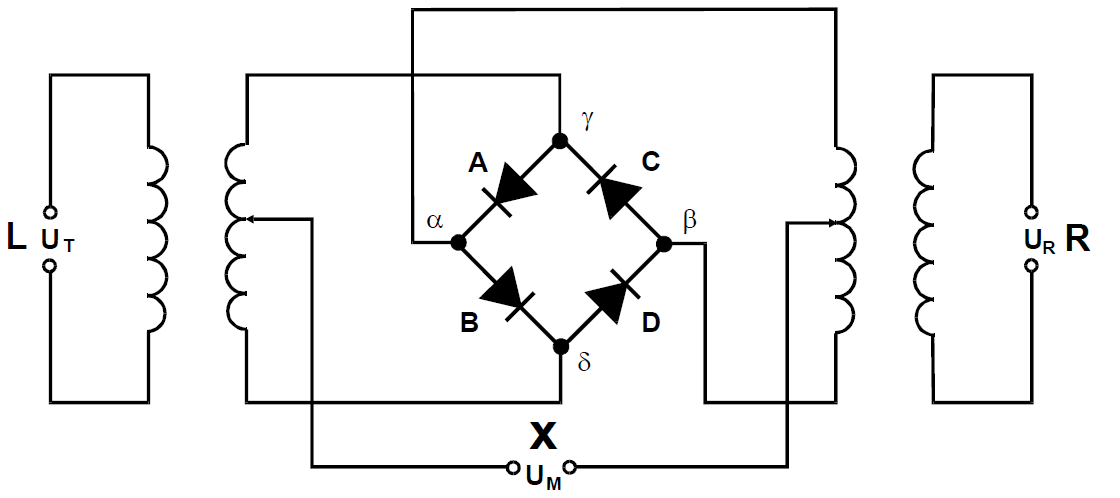
\includegraphics[width=13cm]{images/ringmodulatorschaltung.png}
\caption{Schaltbild eines Ringmodulators (1)}
\label{fig:ringmodulator}
\end{figure} 
Bei idealen Verhältnissen ist
\begin{align}
U_{\text{R}}=\gamma U_{\text{T}}U_{\text{M}}\label{eq:ringmodulatorprodukt}
\end{align}
nur proportional zu den Produkt aus $U_{\text{T}}$ und $U_{\text{M}}$ und es treten nur die beiden Seitenlinien im Frequenzspektrum auf.
\subsubsection*{Frequenzmodulation}
Im folgenden soll ein Frequenzmodulator mit geringem Frequenzhub beschrieben werden.\\
Die Voraussetzungen für ein frequenzmoduliertes Signal wurde im Abschnitt \ref{sec:frequenzmodulation} diskutiert. Es wird jeweils eine amplitudenmodulierte Seitenlinien mit Frequenz $\omega_{\text{T}}-\omega_{\text{M}}$ und $\omega_{\text{T}}+\omega_{\text{M}}$ sowie ein um $90^\circ$ verschobenes Trägersignal benötigt.\\
Im vorherigen Abschnitt wurde mit den Ringmodulator eine Möglichkeit beschrieben, um verlustfrei ein amplitudenmoduliertes Signal mit den benötigten Seitenlinien zu erzeugen. Dieses muss danach noch um den um $90^\circ$ verschobenen Trägersignal ergänzt werden. Dies ist mit der in Abbildung \ref{fig:frequenzmodulationsschaltung} dargestellten Schaltung möglich.
\begin{figure}[H]
\centering 
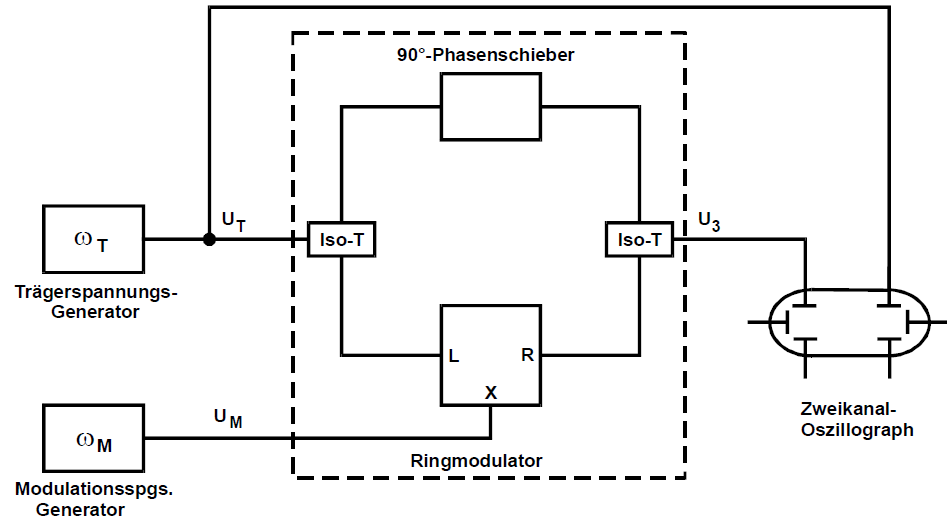
\includegraphics[width=13cm]{images/frequenzmodulationsschaltung.png}
\caption{Schaltbild für einen Frequenzmodulator mit geringem Frequenzhub (1)}
\label{fig:frequenzmodulationsschaltung}
\end{figure} 
\subsection{Demodulator-Schaltungen}
\subsubsection*{Amplitudenmodulierte Signale}
Aus Gleichung \ref{eq:ringmodulatorprodukt} geht hervor, dass ein Ringmodulator das Produkt zweier Spannungen bildet und dabei treten Frequenzen mit $\omega_{\text{T}}-\omega_{\text{M}}$ und $\omega_{\text{T}}+\omega_{\text{M}}$ auf.\\
Um eine Demodulation zu erhalten, wird auf L eine Spannung mit der Frequenz $\omega_{\text{T}}$ angelegt, sodass am Ausgang X eine Spannung mit Frequenzen $\omega_{\text{M}}$, $2\omega_{\text{T}}-\omega_{\text{M}}$ und $2\omega_{\text{T}}+\omega_{\text{M}}$ anliegt. Die störenden Frequenzen können mithilfe eines Tiefpasses herausgefiltert werden, da meistens $\omega_{\text{T}}$ viel größer als $\omega_{\text{M}}$ ist. Nach den Tiefpass kann anschließend ein Signal mit der gewünschten Frequenz $\omega_{\text{M}}$ abgegriffen werden. Der Schaltplan ist in Abbildung \ref{fig:demodulationsschaltungmitringmodulator} dargestellt.\\
Ein Problem dabei ist, dass die Trägerfrequenz für die Demodulation starr mit der Trägerfrequenz der Modulation gekoppelt sein muss. Das Problem kann durch sogenannte Phasenregelkreise umgangen werden.
\begin{figure}[H]
\centering 
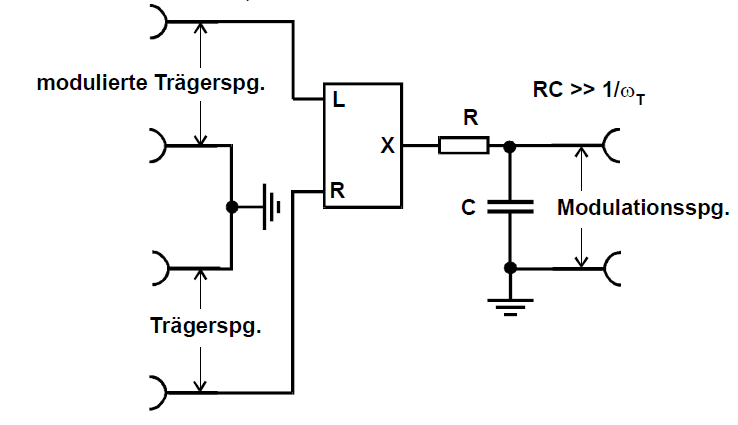
\includegraphics[width=10cm]{images/demodulationsschaltungmitringmodulator.png}
\caption{Demodulator-Schaltung mit einem Ringmodulator (1)}
\label{fig:demodulationsschaltungmitringmodulator}
\end{figure} 
Alternativ kann auch eine Diode zur Demodulation verwendet werden, die nach Abbildung \ref{fig:demodulationsschaltungmitgleichrichtdiode} aufgebaut wird.
\begin{figure}[H]
\centering 
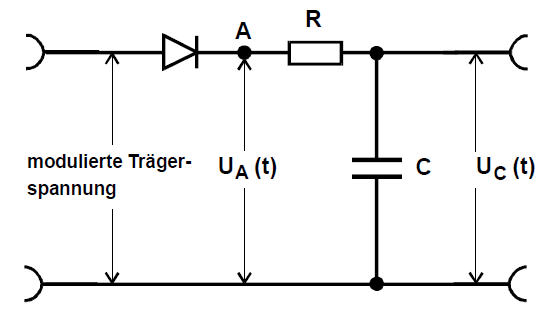
\includegraphics[width=10cm]{images/demodulationsschaltungmitgleichrichtdiode.png}
\caption{Demodulator-Schaltung mit einer Gleichrichter-Diode (1)}
\label{fig:demodulationsschaltungmitgleichrichtdiode}
\end{figure}
Die Diode schneidet sämtliche negative Halbwellen ab, sodass ein Signal der Form wie in der Abbildung \ref{fig:AusgangsspannungDemodulationDiode}.\\
Die hochfrequenten Anteile können mithilfe eines Tiefpasses unterdrücken.\\
Dies funktioniert unter der Annahme, dass die Diode eine lineare Strom-Spannungs-Kennlinie besitzt. Dies ist in der Praxis nicht der Fall, da die Kennlinie einer Halbleiter-Diode näherungsweise Exponentiell, sodass am Ausgang des Demodulators Verzerrungen auftreten.\\
Die Verzerrungen können jedoch in Grenzen gehalten werden, indem der Modulationsgrad gering gehalten wird. \\
Eine weitere Verbesserung der Linearität kann durch die Gegentaktschaltung erreicht werden, bei der beide Halbwellen ausgenutzt werden.
\begin{figure}[H]
\centering 
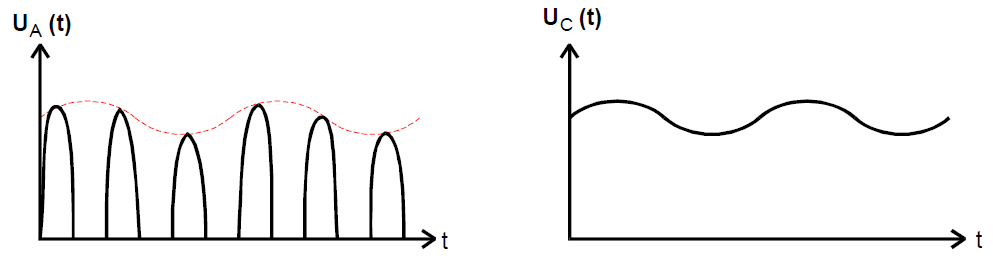
\includegraphics[width=14cm]{images/AusgangsspannungDemodulationDiode.png}
\caption{Gleichgerichtete modulierte Hochfrequenz-Spannung (links) und die dazugehörige Ausgangsspannung der Demodulator Schaltung hinter dem Tiefpass (rechts) (1)}
\label{fig:AusgangsspannungDemodulationDiode}
\end{figure}
\subsubsection*{Frequenzmodulierte Signale}
Die Demodulation eines frequenzmodulierten Signal kann beispielsweise durch einen Flankenmodulator geschehen. Dieser besteht, wie in Abbildung \ref{fig:Flankenmodulator} abgebildet, aus einen Schwingkreis, bei den die Frequenzabhängigkeit der Kondensatorspannung bei angeregten Schwingungen ausgenutzt wird.
\begin{figure}[H]
\centering 
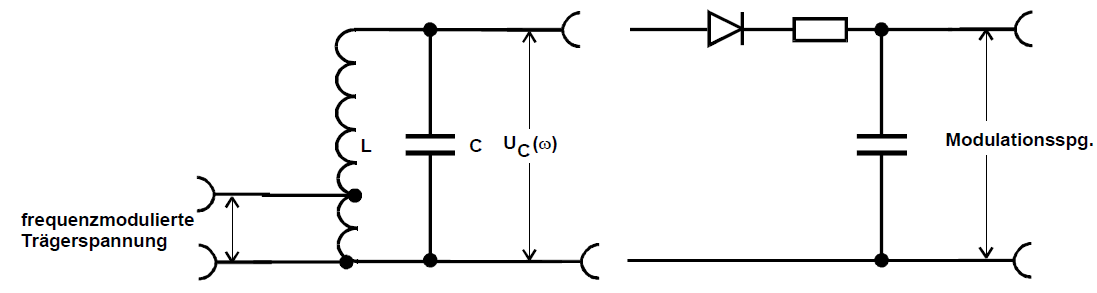
\includegraphics[width=15cm]{images/Flankenmodulator.png}
\caption{Schaltbild eines Eintrakt-Flankenmodulator als Demodulator (1)}
\label{fig:Flankenmodulator}
\end{figure}
Die Resonanzfrequenz des Schwingkreises wird dafür so eingestellt, dass die Trägerfrequenz $\omega_{\text{T}}$ in der steilen Flanke der Resonanzkurve liegt, wie in Abbildung \ref{fig:flanke} abgebildet ist.
\begin{figure}[H]
\centering 
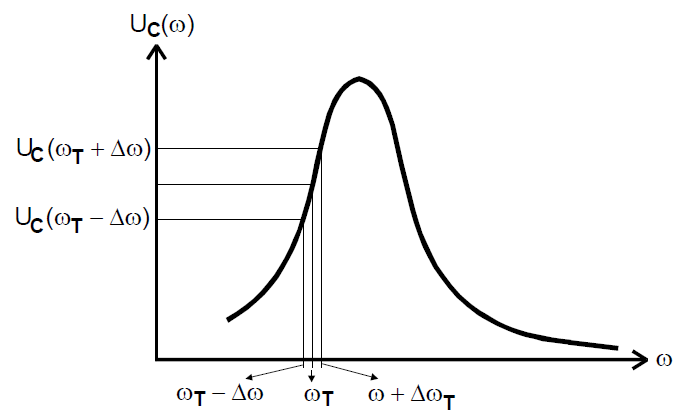
\includegraphics[width=10cm]{images/flanke.png}
\caption{Resonanzkurve des Schwingkreises im Flankendemodulator (1)}
\label{fig:flanke}
\end{figure}
Die Änderung der Momentfrequenz der modulierten Schwingung führt am Ausgang des Schwingkreises zu einer hochfrequenten Spannung $U_\text{c}\left(\omega\right)$, deren Amplitude im Rhythmus der Modulation schwankt. Das frequenzmodulierte Signal wurde so in ein amplitudenmoduliertes Signal überführt, welches mit den vorher besprochenen Methoden demodulieren werden kann.
\section{Durchführung}
Es sollen Schwingungen sowohl amplituden- als auch frequenzmoduliert werden. Dabei sind die folgenden Arbeitsschritte vorgesehen:\\
\begin{itemize}
	\item Mithilfe eines Ringmodulators wird ein amplitudenmoduliertes Signal erzeugt und auf einem Oszilloskop abgebildet. Außerdem wird mit einem Frequenzanalysator das Frequenzspektrum untersucht. \\
	\item Das modulierte Signal wird nun sowohl mit einem weiteren Ringmodulator als auch mit einer Diodenschaltung demoduliert und das Ausgangssignal auf dem Oszilloskop dargestellt. \\
	\item Es wird ein amplitudenmoduliertes Signal mithilfe einer Diodenschaltung erzeugt und mit Oszilloskop und Frequenzanalysator untersucht. \\
	\item Die Cosinus-Abhängigkeit der Ausgangsspannung eines phasenempfindlichen Gleichrichters soll überprüft werden. \\
	\item Es wird ein frequenzmoduliertes Signal erzeugt und auf einem Oszilloskop betrachtet sowie mit dem Frequenzanalysator untersucht. \\
	\item Das frequenzmodulierte Signal wird demoduliert und mit dem Modulationssignal verglichen.
\end{itemize}

\section{Auswertung}

\subsection{Amplitudenmodulation mit Ringmodulator}
Mit einem Ringmodulator wird ein amplitudenmoduliertes Signal mit Trägerunterdrückung erzeugt. Freequenzen f und Amplituden U von Träger- und Modulationssignal lauten:
\begin{itemize}
	\item Trägersignal f$_t=(10.00\pm0.01)$\,MHz, U$=(2.70\pm0.01)$\,V
	\item Modulationssignal f$_m=(158\pm1)$\,kHz, U=$(360\pm1)$\,mV
\end{itemize}
Der Ergebnis der Amplitudenmodulation ist in Abbildung \ref{fig:ampmodring} dargestellt.
\begin{center}
	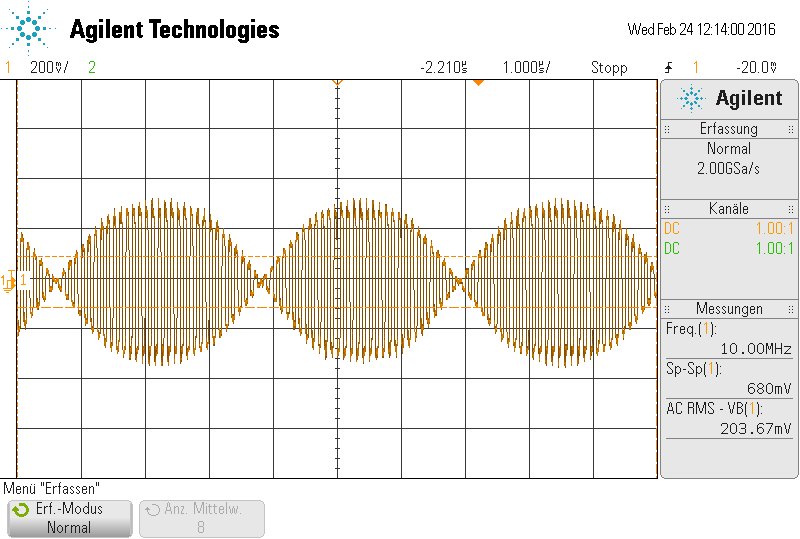
\includegraphics[width=10cm]{images/ampmodring.png}
	\captionof{figure}{Amplitudenmoduliertes Signal, erzeugt mit Ringmodulator}
	\label{fig:ampmodring}
\end{center}
Eine Aufnahme des Frequenzspektrums, welches mit einem Frequenzanalysators aufgenommen wurde, ist in Abbildung \ref{fig:freqampmodring} dargestellt. Der Anteil der Trägerfrequenz ist um zwei Dekaden geringer als die der Seitenbänder.
Mithilfe des Frequenzanalysators können die Frequenzen abgelesen werden:
\begin{itemize}
	\item linkes Seitenband: 9.836\,MHz
	\item mittleres Frequenzband: 9.995\,MHz
	\item rechtes Seitenband: 10.15\,MHz
\end{itemize} 
\begin{center}
	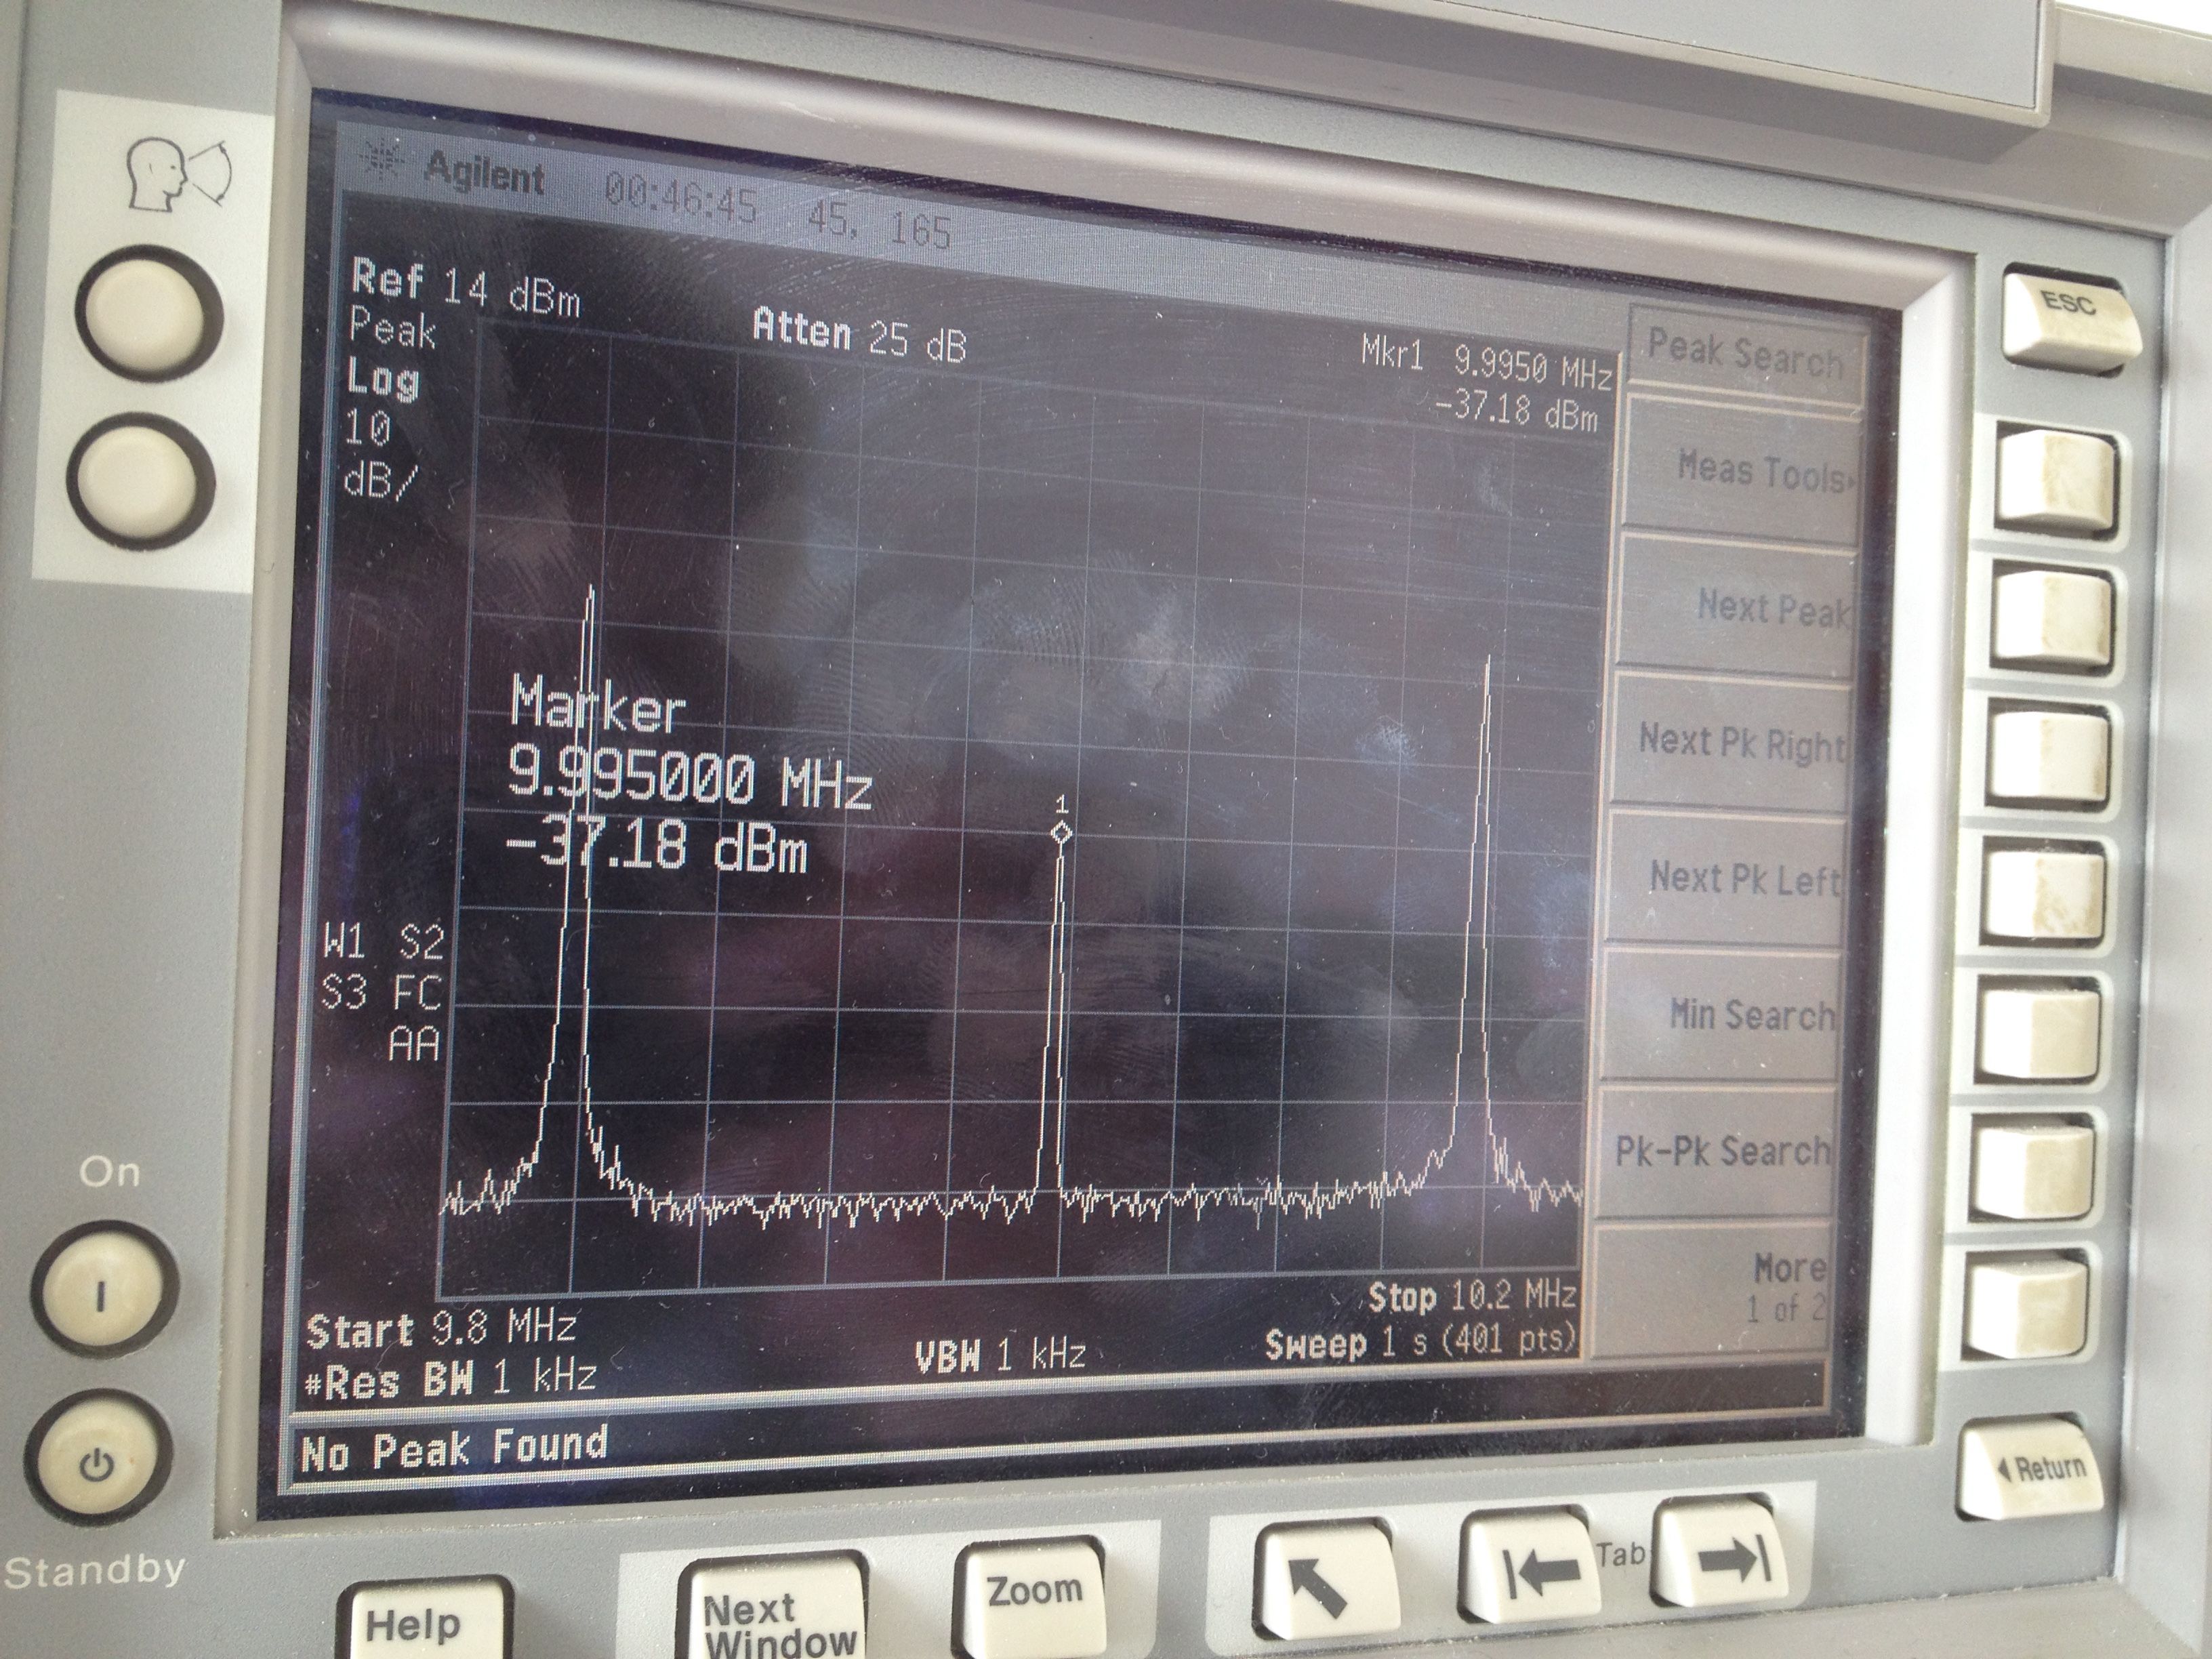
\includegraphics[width=10cm]{images/freqampmodring.jpg}
	\captionof{figure}{Frequenzspektrum eines amplitudenmoduliertes Signals mit einem Ringmodulator, die Trägerfrequenz ist um eine Dekade unterdrückt.}
	\label{fig:freqampmodring}
\end{center}
%Bis hierhin verbessert
\subsection{Ausmessung des phasenempfindlichen Gleichrichters}
Bevor die Amplitudendemodulation vorgenommen wird, wird zunächst der phasenempfindliche Gleichrichter ausgemessen und untersucht, ob die Ausgangsspannung der Relation
\begin{align}
U_{\text{ph}}=a\cos(\phi+b)
\label{eq:phasen}
\end{align}
folgt, wobei $\phi$ dabei die Phasendifferenz der beiden Eingangssignale darstellt. \\\
Die Phasendifferenzen $\phi$ werden über eine variable Verzögerungsleitung eingestellt, wodurch sich die Phasendifferenzen $\phi$ aus 
\begin{align}
\phi = tf2\pi
\end{align}
ergibt, mit f der Frequenz und t der Verzögerungszeit. Dazu wird die Frequenz auf f=9.58\si{MHz} eingestellt, um ein möglichst großes Intervall für die Phasendifferenz abzudecken. Die aufgenommenen Messwerte sind in Tabelle \ref{tab:phasen} dargestellt. \\
\begin{center}
	\begin{tabular}{|c|c||c|c|}
		\hline $\Delta$t [ns] & U [V] & $\Delta$t [ns] & U [V]\\
		\hline	0	&	-0,247	&	32	&	0,17	\\
		\hline	1	&	-0,239	&	40	&	0,238	\\
		\hline	2	&	-0,231	&	48	&	0,263	\\
		\hline	4	&	-0,215	&	56	&	0,21	\\
		\hline	8	&	-0,175	&	64	&	0,127	\\
		\hline	16	&	-0,072	&	72	&	0,003	\\
		\hline	18	&	-0,038	&	80	&	-0,114	\\
		\hline	19	&	-0,02	&	88	&	-0,205	\\
		\hline	20	&	-0,006	&	96	&	-0,261	\\
		\hline	24	&	0,061	&	104	&	-0,242	\\
		\hline	28	&	0,117	&	112	&	-0,17	\\
		\hline	30	&	0,143	&		&	\\	
		\hline
	\end{tabular}
	\captionof{table}{Aufgenommene Messwerte für Verzögerungszeit $\Delta$t und Spannung zur Vermessung des phasenempfindlichen Gleichrichters}
	\label{tab:phasen}
\end{center}
Mithilfe von Python werden die Verzögerungszeiten in Phasendifferenzen umgerechnet und eine nicht-lineare Ausgleichsrechnung durchgeführt, mithilfe von Gleichung \ref{eq:phasen}. Der entsprechende Plot ist in Abbildung \ref{fig:phasen} dargestellt, die nicht-lineare Ausgleichsrechnung ergibt dabei die folgenden Parameter:
\begin{align}
a &= (-0.259 \pm 0.001) V \\
b &= ( 0.352 \pm 0.004) 
\end{align}
\begin{center}
	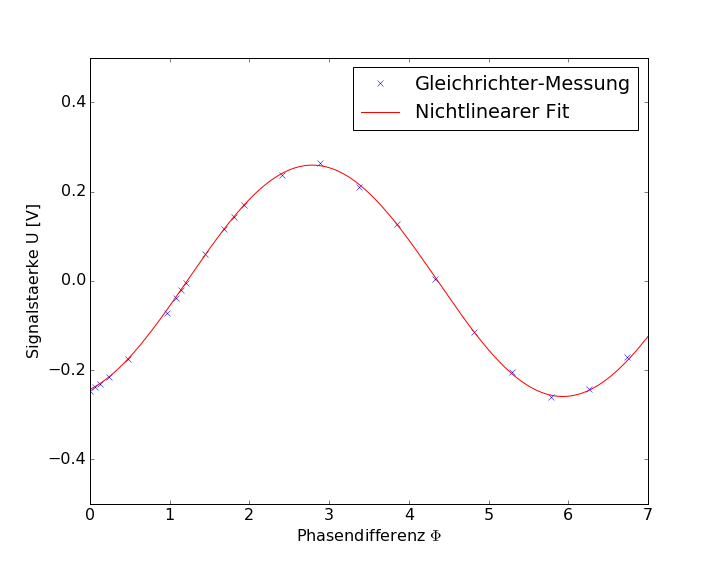
\includegraphics[width=10cm]{images/plotgleich.png}
	\captionof{figure}{Messwerte für den phasenabhängigen Gleichrichter und Cosinus-Fit für diese.}
	\label{fig:phasen}
\end{center}
Es zeigt sich ein Cosinus-Verhalten der Ausgangsspannung in Abhängigkeit von der Phasendifferenz.

\subsection{Amplitudendemodulation mit Ringmodulator}
Das zuvor mit einem Ringmodulator modulierte Signal wird nun mit einem weiteren Ringmodulator demoduliert. Das Eingangssignal und das Signal am Ausgang des zweiten Ringmodulators ist in Abbildung \ref{fig:ampdemodring} dargestellt.
\begin{center}
	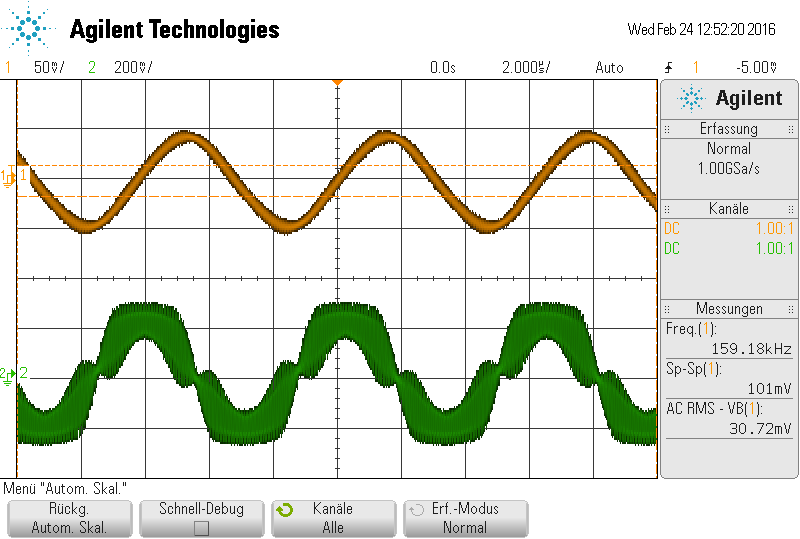
\includegraphics[width=10cm]{images/ampdemodring.png}
	\captionof{figure}{Eingangssignal (oberes Singal) und demoduliertes Signal (unteres Signal), welches am Ausgang des zweiten Ringmodulators gemessen wird.}
	\label{fig:ampdemodring}
\end{center}

\subsection{Amplitudendemodulation mit Diode}
Das amplitudenmodulierte Signal wird nun mithilfe einer Gleichrichterdiodenschaltung demoduliert. Das Ergebnis dieser Demodulation ist in Abbildung \ref{fig:ampdemoddio} dargestellt. 
\begin{center}
	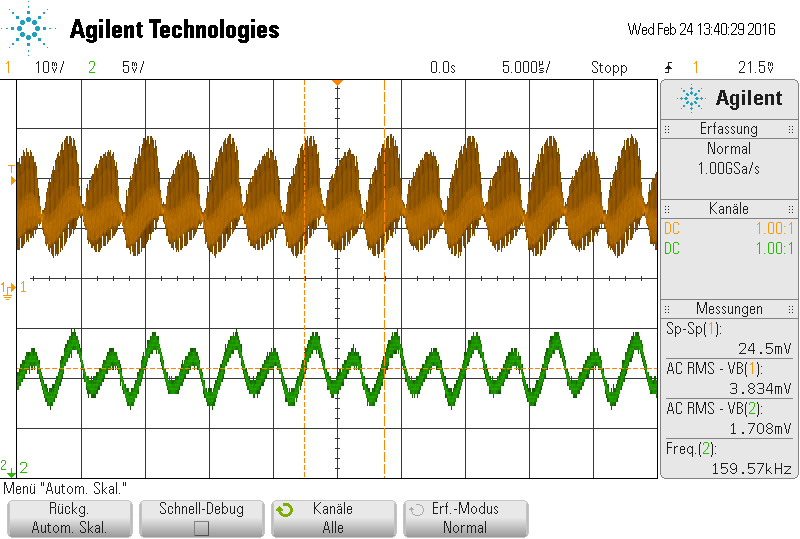
\includegraphics[width=10cm]{images/ampdemoddio.png}
	\captionof{figure}{Das obere Signal wird am Punkt A direkt nach der Gleichrichterdiode abgegriffen, das zweite Signal ist das demodulierte Signal, welches hinter dem Tiefpass abgegriffen wird.}
	\label{fig:ampdemoddio}
\end{center}
Zur\subsection{Amplitudenmodulation mit Diode}
Auch mit einer Diode kann ein Signal amplitudenmoduliert werden. Dabei kommt es zur Trägerabstrahlung. Der Signalverlauf nach der Amplitudenmodulation ist in Abbildung \ref{fig:ampmoddio} dargestellt. \\
Es soll der Modulationsgrad m aus der Abbildung ermittelt werden. Dieser bestimmt sich aus
\begin{align}
m=\frac{U_{max}-U_{min}}{U_{max}+U_{min}}\,.
\label{eq:modgrad}
\end{align}
\begin{center}
	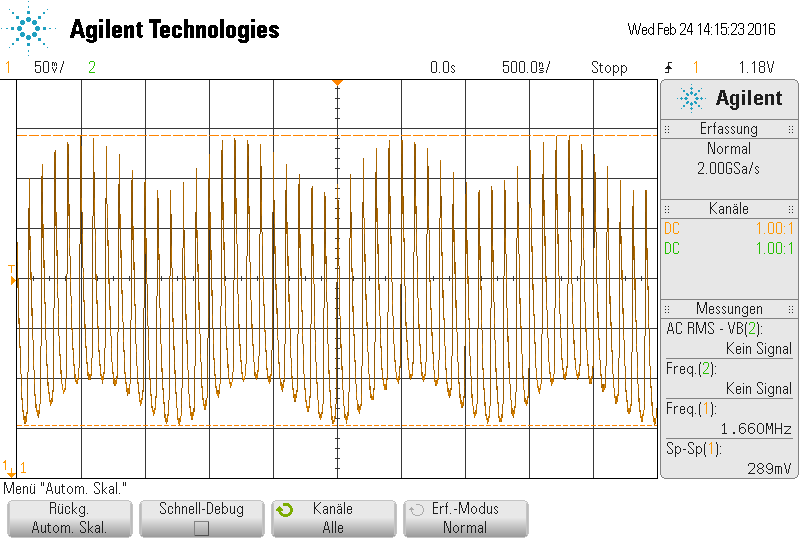
\includegraphics[width=10cm]{images/ampmoddio.png}
	\captionof{figure}{Mittels einer Diodenschaltung erzeugte amplitudenmoduliertes Signal.}
	\label{fig:ampmoddio}
\end{center}
Aus der Abbildung werden maximale und minimale Spannung abgelesen:
\begin{align*}
\text{U}_{\text{max}}=(0.290\pm 0.05)\si{V} \\
\text{U}_{\text{min}}=(0.160\pm 0.05)\si{V}
\end{align*}
Dies ergibt ein Modulationsgrad von $m=0.29\pm0.16$. Die Fehlerrechnung wurde mithilfe des Python-Paketes 'uncertainties' durchgeführt. \\
Aus dem aufgenommenen Frequenzspektrum kann ebenfalls der Modulationsgrad entnommen sowie die Oberschwingungen des Trägers erkannt werden. \\
\begin{center}
	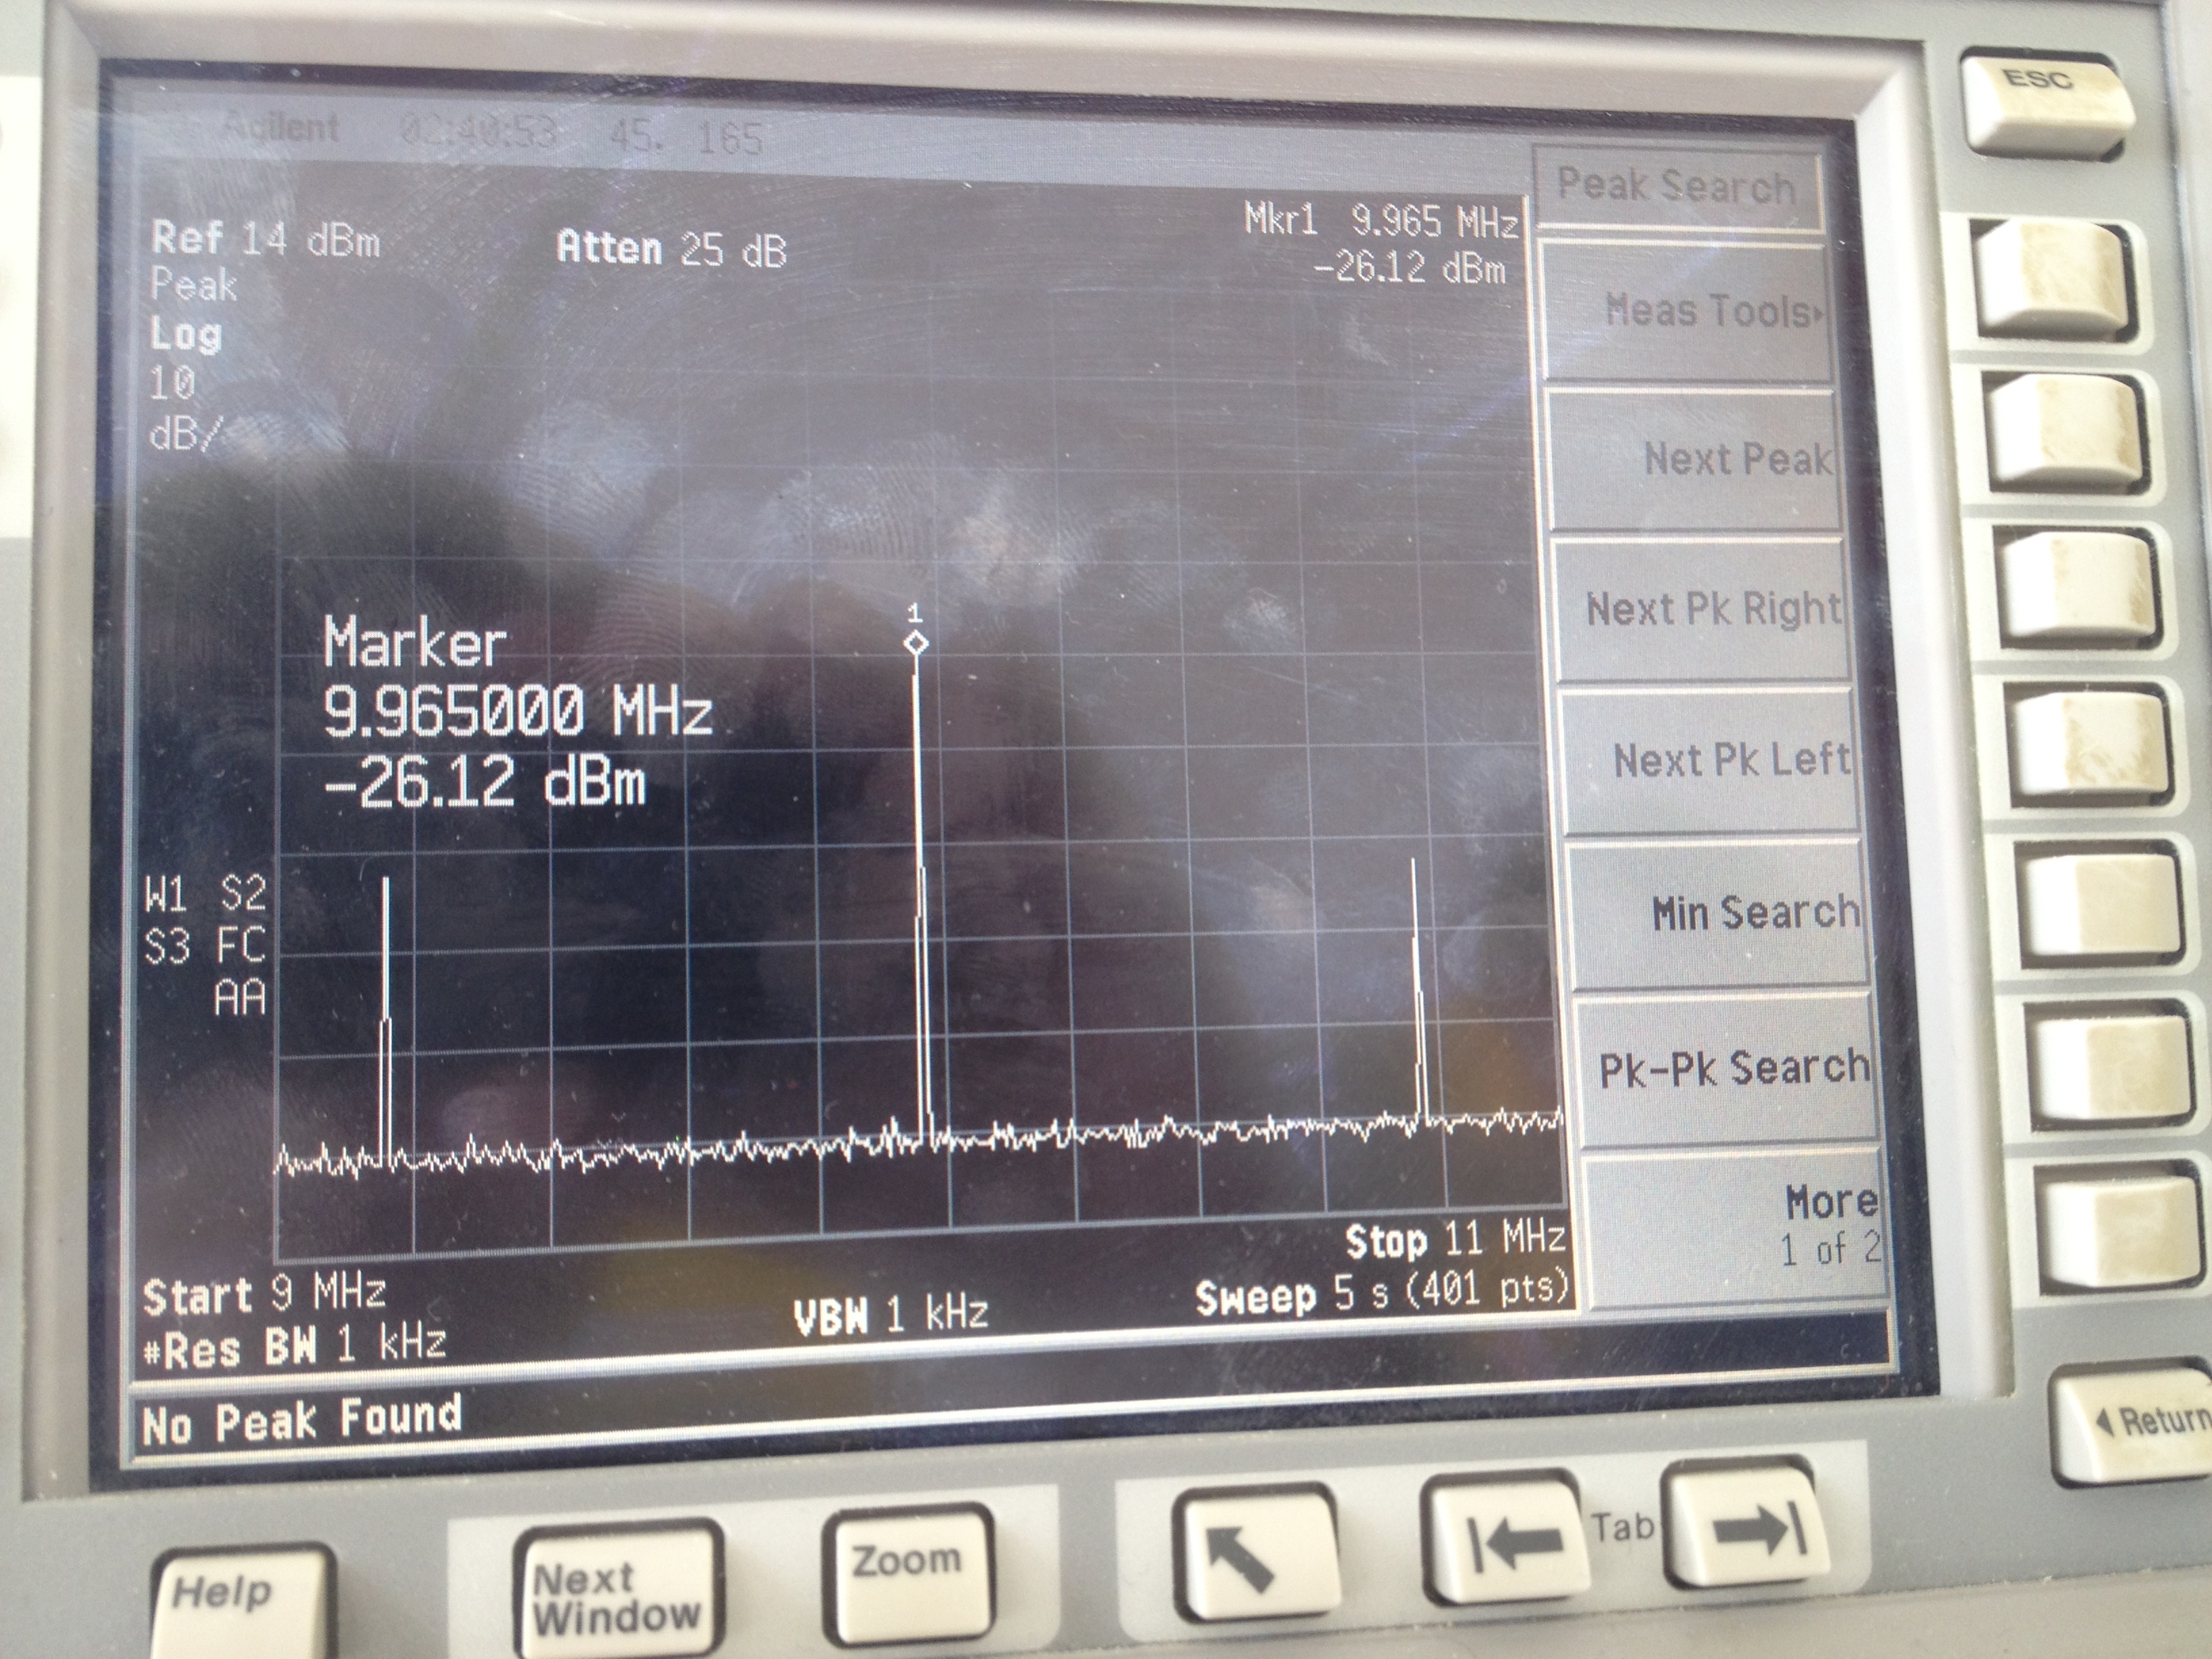
\includegraphics[width=10cm]{images/freqampmoddio.jpg}
	\captionof{figure}{Frequenzspektrum des mit Diodenschaltung amplitudenmodulierten Signals. Es ist deutlich zu erkennen, dass keine Trägerunterdrückung vorliegt.}
	\label{fig:freqdio}
\end{center}
\begin{center}
	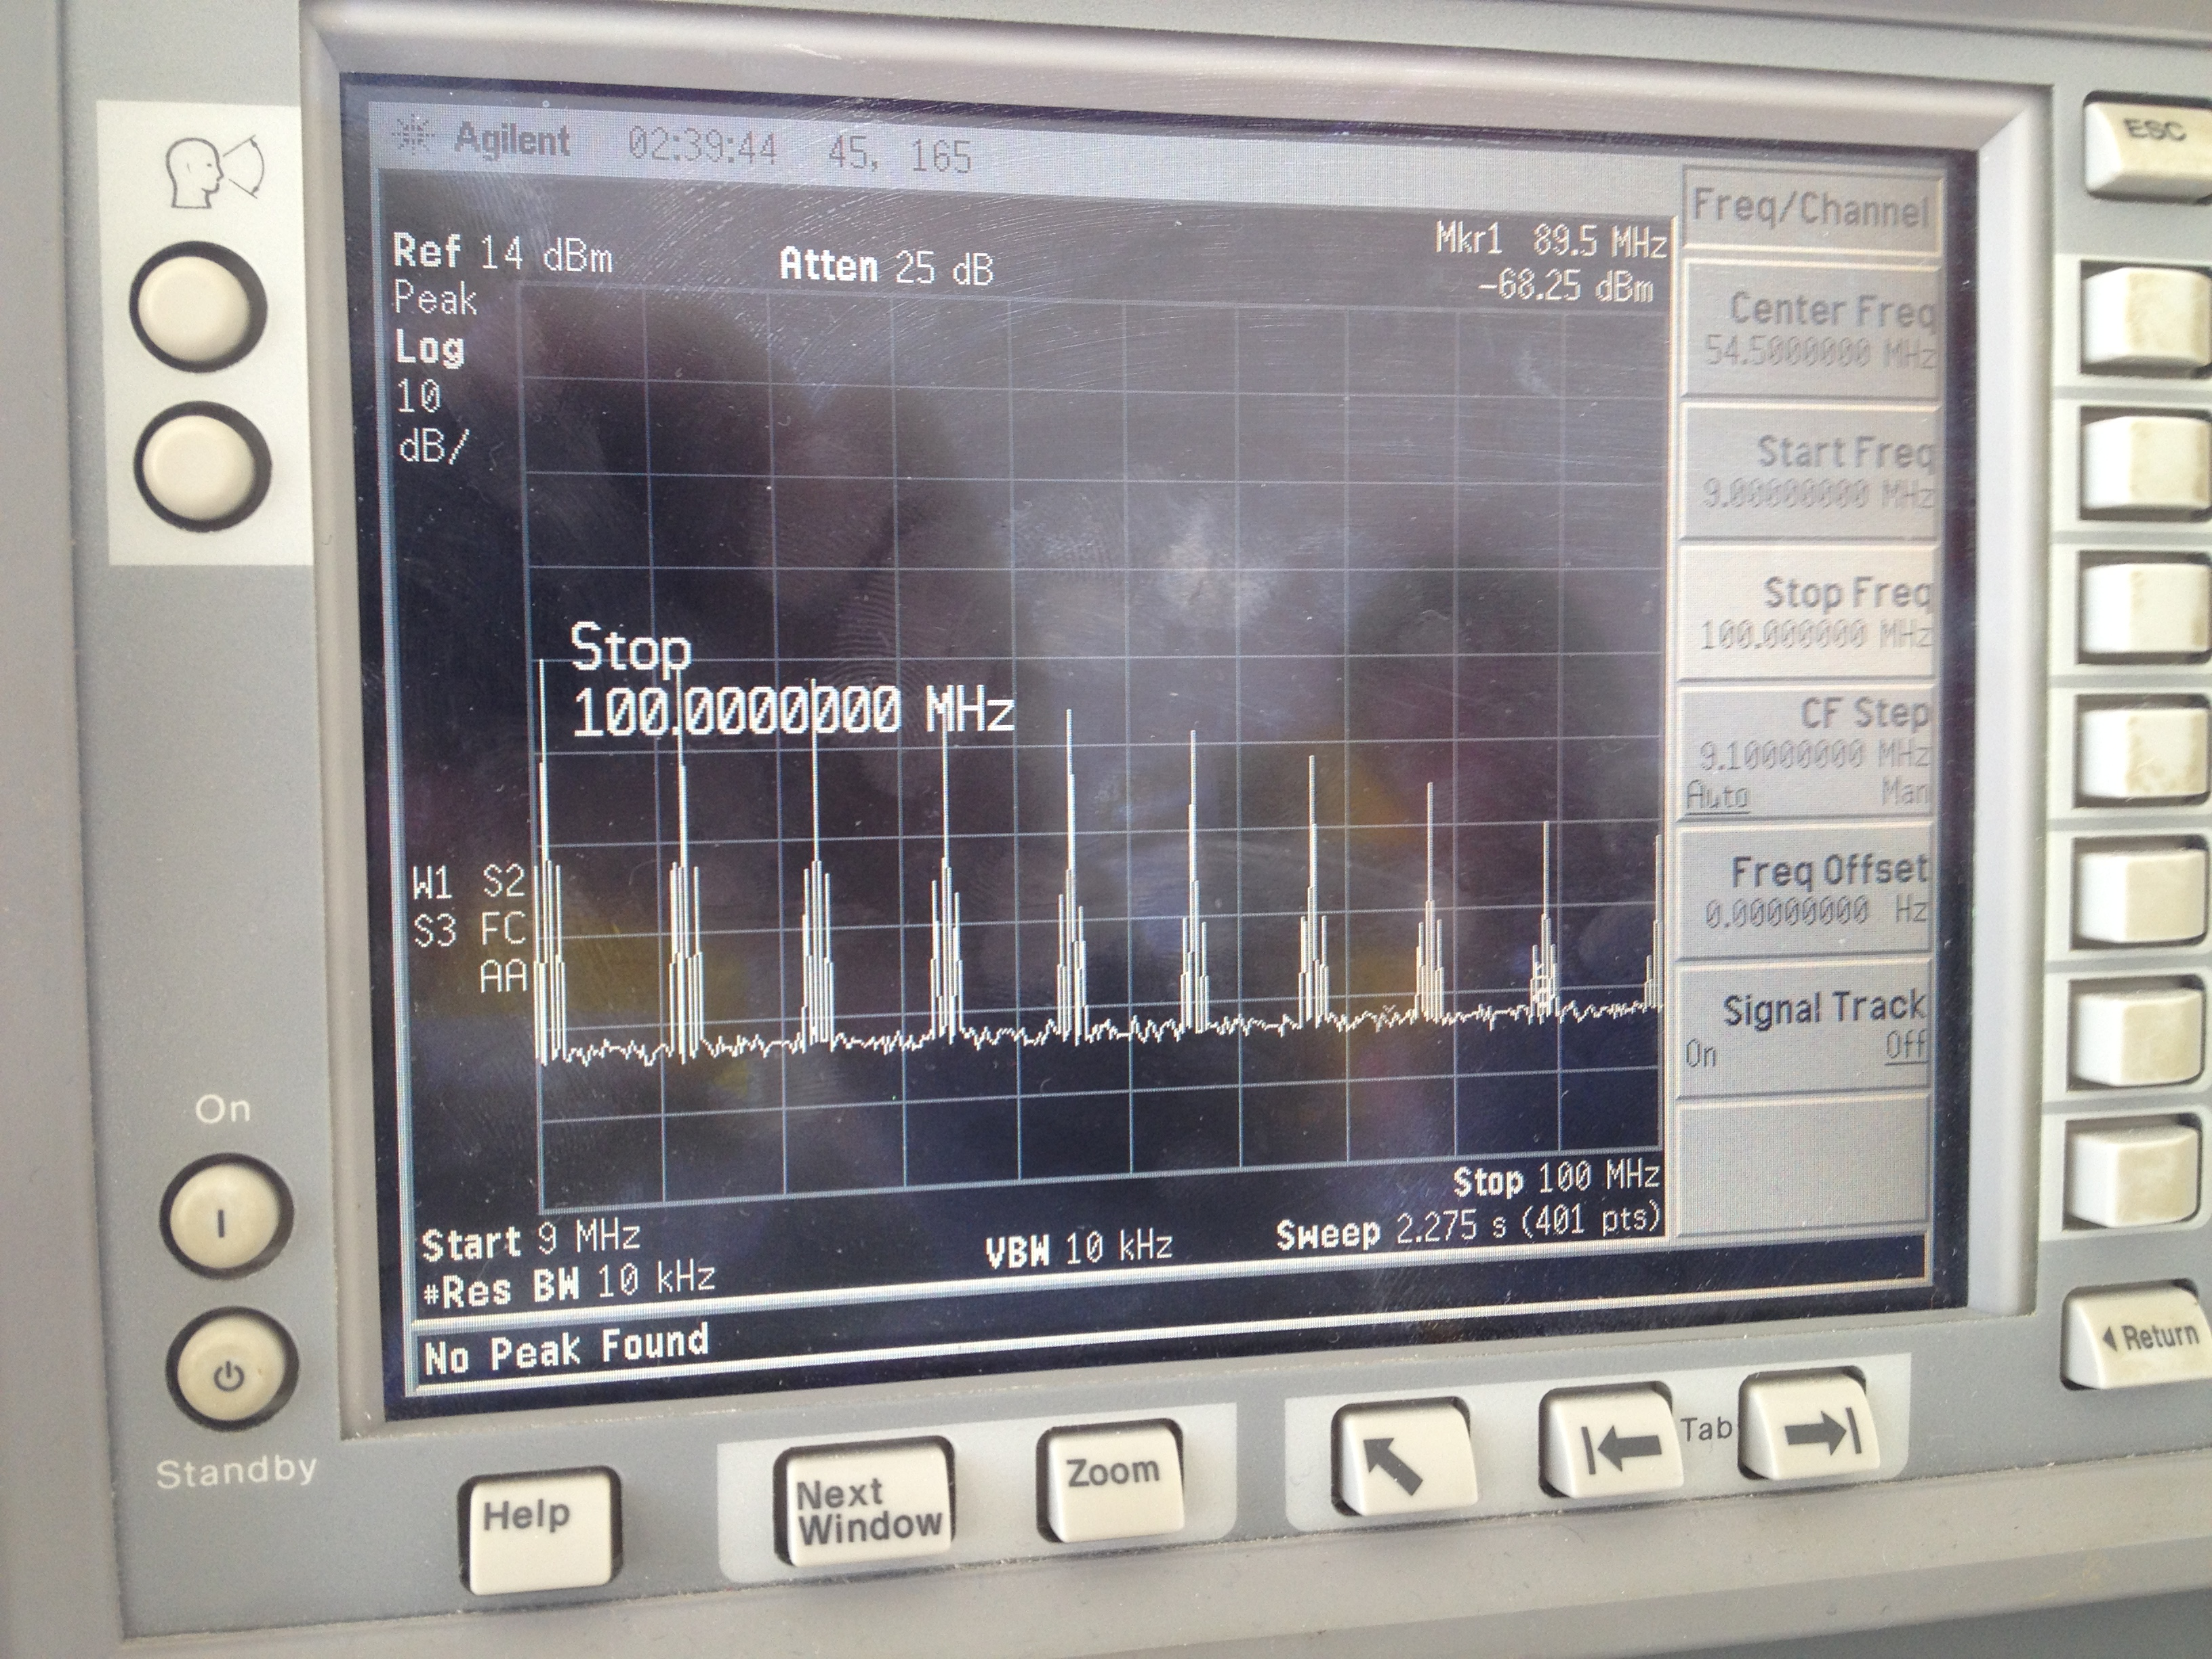
\includegraphics[width=10cm]{images/oberwellen.jpg}
	\captionof{figure}{Frequenzspektrum des amplitudenmodulierten Signals über einen größeren Frequenzbereich. Die Oberwellen des Signals können gut erkannt werden.}
	\label{fig:oberwellen}
\end{center}
Der Modulationsgrad m ergibt sich aus den Amplituden der Träger- und der Modulationsspannung, wobei diese Werte abgelesen werden können.Dabei wurde die Messfunktion des Frequenzanalysators verwendet. Es muss eine Umrechnung von dBm-Skala in lineare Skala stattfinden. \\
Der Modulationsgrad berechnet sich somit aus
\begin{align}
\text{A}=10^{\frac{W}{20}} \\
\text{m}=2\frac{A_M}{A_T}\,.
\end{align}
Es ergibt sich:
\begin{itemize}
	\item Trägersignal U$_T=(-26.12\pm 0.01) \text{dbm}$
	\item Modulationssignal U$_M=(-48.67\pm 0.01) \text{dbm}$
	\item Modulationsgrad m$=0.15\pm 0.01$
\end{itemize}

\subsection{Frequenzmodulation}
Zur Erzeugung des frequenzmodulierten Signals wird auf das amplitudenmodulierte Signal ein um $\pi/2$ phasenverschobenes Signal gegeben. Die Phasenverschiebung wird mit einer Frequenz von 1 MHz un einer Verzögerungszeit von $\Delta$t=1000\,. erreicht. Die Phasenverschiebung kann mithilfe der in Abbildung \ref{fig:lisajous} dargestellten Lisajous-Figur überprüft werden. \\
\begin{center}
	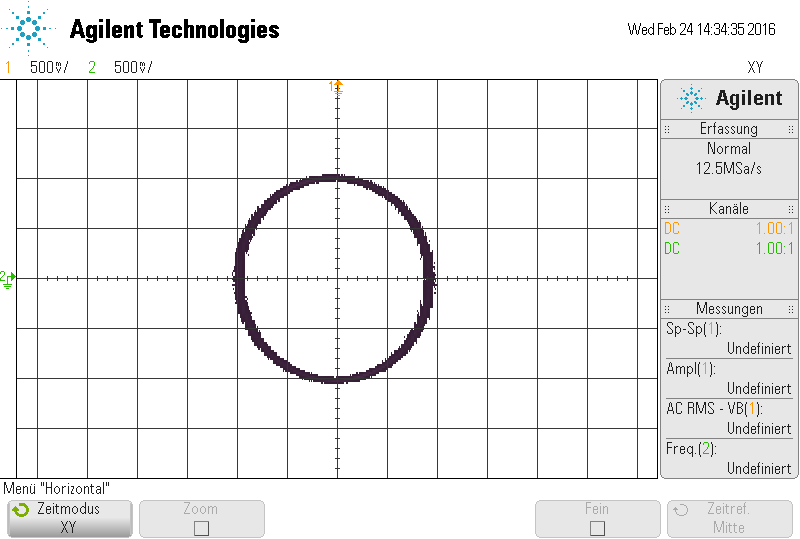
\includegraphics[width=10cm]{images/lisajous.png}
	\captionof{figure}{Lisajous-Figur zur Phasenverschiebung von $\pi/2$. Dabei wurden die beiden Signale im xy-Betrieb des Oszilloskops angezeigt.}
	\label{fig:lisajous}
\end{center}
Mithilfe der Verbreiterung des Signals $\Delta$t nach einer Periode kann der Modulationsgrad m aus
\begin{align}
\Delta\text{t}&=\frac{1}{f_1}-\frac{1}{f_2}=\frac{2\pi}{\omega_T(1-m)}-\frac{2\pi}{\omega_T(1+m)} \\
m&=-\frac{2}{\Delta tf_T}+\sqrt{\frac{2}{(\Delta tf_T)^2}+1}
\end{align}
berechnet werden. \\
Mit dem bekannten Wert $f_T=1$\,MHz und dem abgelesenen Wert $\Delta$t=(375$\pm$ 25)\,ns ergibt sich der Modulationsgrad zu m=$(0.18\pm 0.01)$.
Das entstehende Signal ist in Abbildung \ref{fig:freqmod} dargestellt.
\begin{center}
	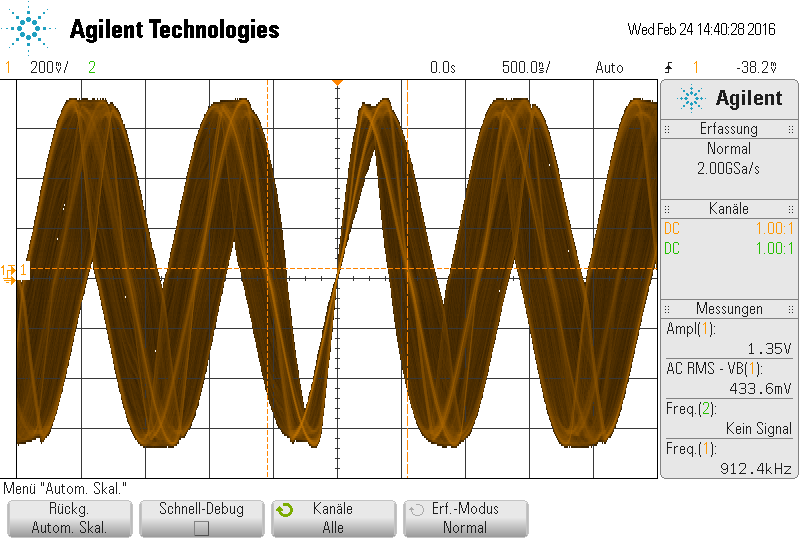
\includegraphics[width=10cm]{images/freqmod.png}
	\captionof{figure}{Ausgangssignal des Frequenzmodulators}
	\label{fig:freqmod}
\end{center}
\begin{center}
	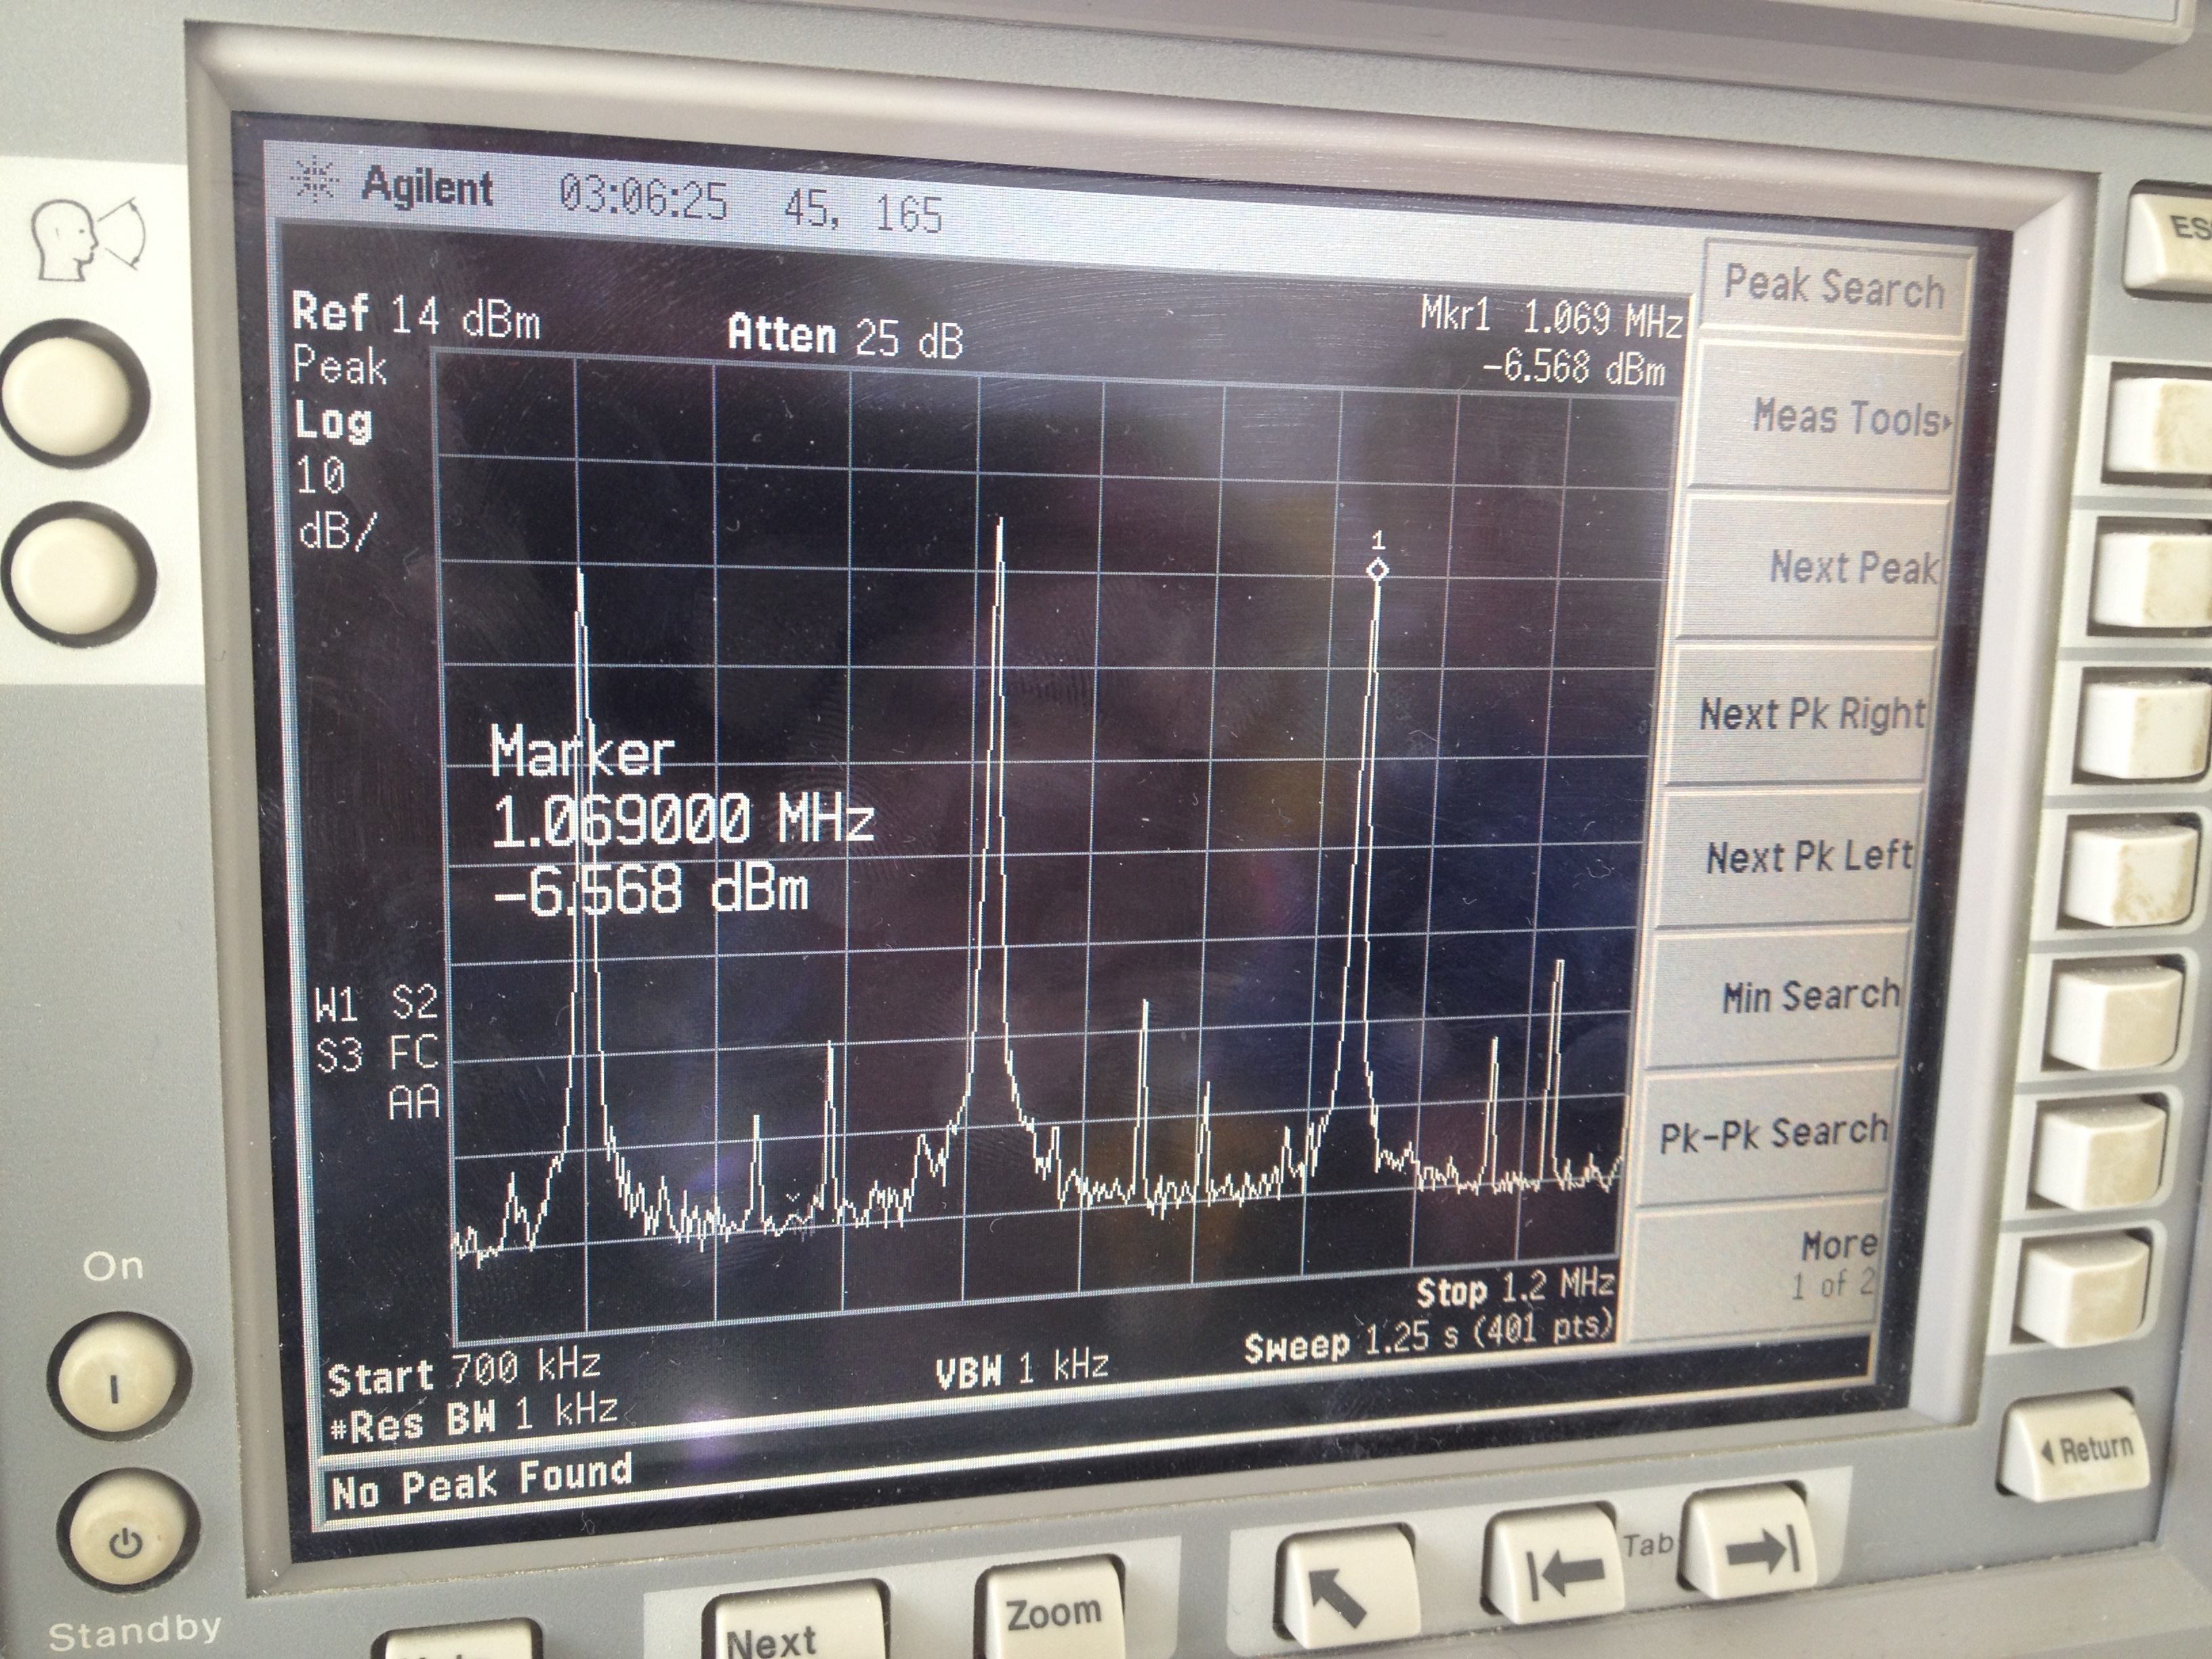
\includegraphics[width=10cm]{images/freqmodfreq.jpg}
	\captionof{figure}{Frequenzspektrum des frequenzmodulierten Signals. Das Trägersignal ist gut zu erkennen.}
	\label{fig:freqmodfreq}
\end{center}
\subsection{Frequenzdemodulation}
Im letzten Versuchsschritt wird das frequenzmodulierte Signal mit einem LC-Kreis und einem Tiefpass demoduliert. Abbildung \ref{fig:lc} zeigt das Signal, wenn es nach dem LC-Kreis abgegriffen wird, Abbildung \ref{fig:tiefpass} zeigt das Signal nach dem Durchlaufen des Tiefpasses. \\
\begin{center}
	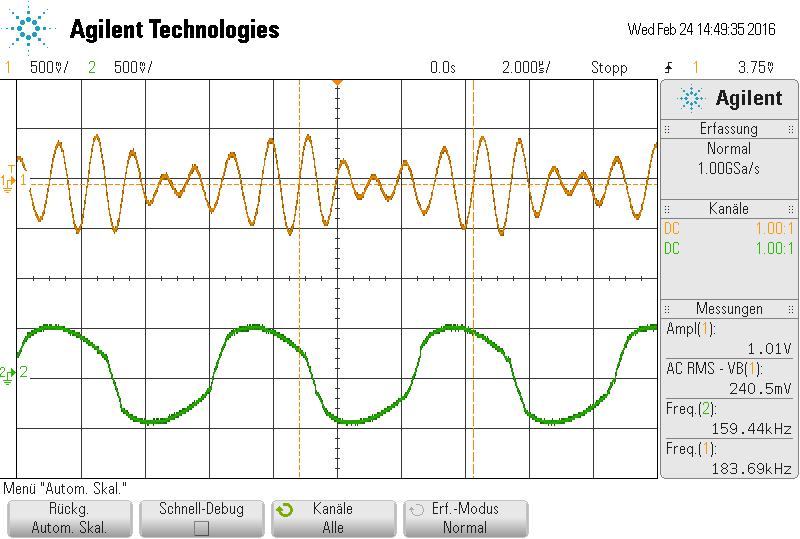
\includegraphics[width=10cm]{images/lc.png}
	\captionof{figure}{Oben ist das Signal direkt nach dem LC-Kreis dargestellt, welches jetzt amplitudenmoduliert ist. Unten ist das Modulationssignal zu sehen.}
	\label{fig:lc}
\end{center}
\begin{center}
	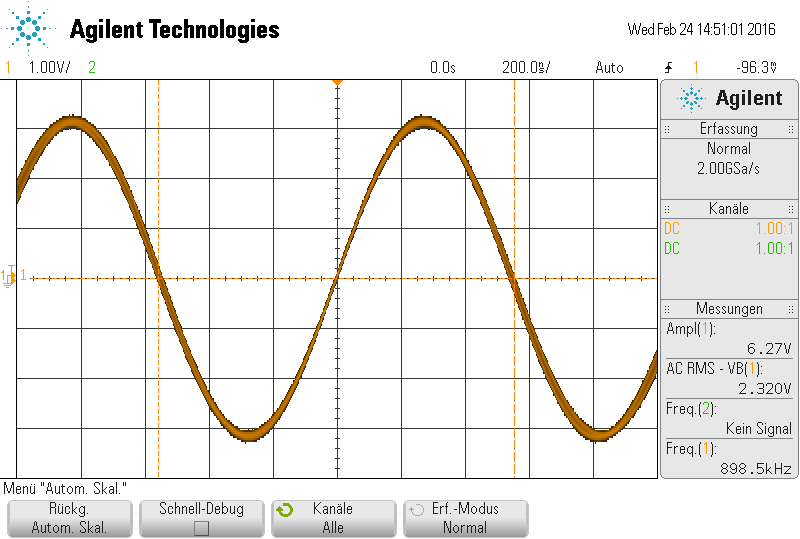
\includegraphics[width=10cm]{images/tiefpass.png}
	\captionof{figure}{Signal nach dem Tiefpass.}
	\label{fig:tiefpass}
\end{center}
\section{Diskussion}
Die erhaltenen Ergebnisse sollen nun hier abschnittsweise diskutiert werden.

\subsection{Amplitudenmodulation mit Ringmodulator}
Das modulierte Signal zeigt das erwartete Verhalten eines amplitudenmodulierten Signales. Im Frequenzspektrum ist deutlich zu erkennen, dass die Trägerfrequenz unterdrückt ist.

\subsection{Ausmessung des phasenempfindlichen Gleichrichters}
Die aufgenommenen Daten bestätigen klar die Cosinus-Abhängigkeit der Ausgangsspannung. Die Fehler der durch den Fit ermittelten Parameter sind gering.

\subsection{Amplitudendemodulation mit Ringmodulator}
Der Vergleich von Eingangssignal und demoduliertem Signal zeigt, dass ein Ringmodulator zur Demodulation von modulierten Signalen geeignet sind. Das Ausgangssignal ist dabei phasenerschoben und verschmiert, stimmt jedoch ansonsten gut mit dem Eingangssignal überein. 

\subsection{Amplitudendemodulation mit Diode}
Die Demodulation mit Diodenschaltung kann das Eingangssignal in grober Näherung wieder reproduzieren. Jedoch kommt es zu Schwankungen in der Amplitude sowie zu Verformungen des Signals. Die Frequenz des Ausgangssignals f=159.57\,kHz weicht jeodoch nur um 1.0\% von der Frequenz des Eingangssignals f=158\,kHZ ab.

\subsection{Amplitudenmodulation mit Diode}
Das amplitudenmodulierte Signal weist keine Trägerunterdrückung auf, wie in Abbildung \ref{fig:freqdio} zu sehen ist. Die erwarteten Oberwellen sind in Abbildung \ref{fig:oberwellen} zu sehen.

\subsection{Frequenzmodulation}
Der berechnete Modulationsgrad ist sehr gering, weist dafür aber nur einen geringen Fehler auf. Das Trägersignal ist gut auf dem Frequenzspektrum zu sehen.

\subsection{Frequenzdemodulation}
Der LC-Kreis wandelt das Signal in ein amplitudenmoduliertes Signal um, was in Abbildung \ref{fig:lc} gut zu sehen ist. Die Frequenz des Ausgangssingnals nach dem Tiefpass weicht jedoch um 11.6\% von der Frequenz des Eingangssignals ab.

\section{Quellen}
{[1]} Versuchsanleitung zu Versuch 59: \\
http://129.217.
224.2/HOMEPAGE/PHYSIKER/MASTER/SKRIPT/V59.pdf (letzte Version vom 30.05.2016, 10:50)\\
\end{document}